\chapter{Implementierung}

\section{Einleitung}

Ziel dieser Arbeit war es, eine Simulationsumgebung für Sensorknoten zu schaffen. Es sollte viele verschiedene Arten von Sensorknoten geben, die jeweils einen oder mehrere verschiedene Sensoren besitzen. Mit diesen Knoten sollte ein Netzwerk aufgebaut werden, um die Umgebungsparameter eines Gebietes zu erfassen.
Die Daten der Simulation sollten visualisiert und ausgewertet werden können, besonders was den Energieverbrauch und die dazugehörigen Batteriezustände im Verlauf der Zeit angeht.

\section{Aufbau und Struktur}

\subsection{Klassenübersicht}

Die Klassenübersichten wurden teilweise mit Hilfe von doxygen\cite{doxygen} erstellt. 

\begin{table}[!ht]
  \centering
  \caption{Klassenübersicht}
  \label{Klassenübersicht}
\begin{tabularx}{\textwidth}{ll}
	\toprule
	Klasse & Beschreibung \\
	\midrule\midrule
	AbstractBatteryAccess &	\specialcell{gibt einer Klasse, welche von dieser erbt Zugriff auf \\die Batterie} \\\midrule
AbstractMemory & \specialcell{eine einfache Implementierung eines \\key-value-Speichers mit CRUD-Operationen}\\\midrule
AbstractProcessor	& \specialcell{Repräsentiert ein paar Grundfunktionen eines \\ Prozessor übernimmt die Steuerung der Sensoreinheit, \\ hat Zugriff auf den Speicher und  kann \\außerdem zwischen verschiedenen power-Modi wechseln }\\\midrule
AbstractSensingUnit & \specialcell{einfache Implementierung einer SensingUnit \\ diese kann Werte der Umgebung messen und \\verbraucht dabei Energie}\\\midrule
AbstractSensorNode	& \specialcell{ist hauptsächlich für die Initialisierung zuständig}\\\midrule
AbstractSignalConditioner	& modelliert den Energieverbrauch vom SignalConditioner \\\midrule
AbstractSignalConverter	& modelliert den Energieverbrauch vom SignalConverter\\\midrule
AbstractTransducer	& modelliert den Energieverbrauch vom Transducer\\\midrule
CustomWorldUtility	& \specialcell{stellt die Umgebung dar:\\ generiert Umweltparameter und speichert diese\\ liefert auf Anfrage von Sensoren Messwerte}\\\midrule
ExtendedMessage & Nachricht mit einigen Parameters für Statistiken\\\midrule
SimpleSensorData	& \specialcell{eine Klasse die von cNamedObject erbt\\ kann eingesetzt werden um an die Parameterliste \\von Nachrichten angehängt zu werden\\mit dieser können Integerwerte versendet werden}\\\midrule
StatisticsInterface & Interface welches Statistiken zur Verfügung stellt\\
	\bottomrule
\end{tabularx}
\end{table}

\subsubsection{CustomWorldUtility}

Die Klasse CustomWorldUtility ist eine sehr wichtige für die Simulation. Sie repräsentiert die Umgebung, also den Bereich indem sich die Knoten befinden. Sie erbt von der Klasse BaseWorldUtility aus dem MiXiM-Framework. BaseWorldUtility stellt die nötigen Funktionalitäten für den sogenannten Playground bereit. \newline
Zusätzlich dazu stellt die Klasse selbst die notwendigen Parameter für die Umwelt bereit. Nach dem Starten der Simulation steht darin jeweils ein k-dimensionales Array pro Sensortyp bereit: temperatureArray, pressureArray, humidityArray und lightArray. Dabei ist k die definierte Anzahl der Dimensionen, jenachdem ob eine 2-dimensionale Fläche oder ein 3-dimensionaler Raum simuliert werden soll. Die Arrays enthalten die Parameter der Umgebung; temperatureArray beinhaltet zum Beispiel, wie der Name schon sagt, Informationen über die Temperatur. \newline
Es kann zu Beginn der Simulation entschieden werden, ob neue Werte berechnet werden sollen oder die bereits vorhandenen Werte für die Umgebung übernommen werden sollen. Die Arrays besitzen die gleiche Größe wie der Playground. Diese Größe ist auch zusätzlich in den Parametern sizeX, sizeY und sizeZ gespeichert. \newline
Da jedoch im 3-dimensionales Fall die Datenmenge sehr schnell steigt, ist auch möglich über den Paremeter dataGranularity im zugehörigen ned-Modul zu definieren, wie detailliert die Daten erstellt werden sollen. Sollte man zum Beispiel den Wert 10 setzen, so wird nur alle 10 Meter ein Wert generiert.\\
Wenn neue Werte generiert werden sollen, so wird für jeden Messtyp eine xml-Datei in der entsprechenden Größe angelegt und mit Messdaten gefüllt. Diese werden anschließend ausgelesen und in Form der oben genannten Arrays gespeichert. Wenn keine neuen Daten erstellt werden sollen, so wird ein bereits existierendes xml-File genutzt.\\
Zum Erstellen neuer Daten kann die Funktion \textbf{generateEnvironmentData()} genutzt werden. Es ist dadurch auch möglich während der Simulation neue Werte zu generieren, indem man diese Funktion aufruft. Die Funktion legt pro Umweltparameter eine xml-Datei im Ordner \textit{WorldModel/data} an. Jede der xml-Dateien wird beim Start mit Hilfe der Funktion \textbf{readXML(int)} eingelesen, verarbeitet, das heißt in ein Array umgewandelt und anschließend in der Klasse gespeichert. \newline
Sollte nun ein Sensor einen Messwert auslesen wollen, so kann dieser auf die Funktion \textbf{getValueByPosition((std::string type, Coord *position))} zugreifen und anhand seines Sensortyps und seiner Position einen entsprechenden Wert geliefert bekommen.

\paragraph{Einblick in einige Funktionen}

Wie im vorigen Abschnitt beschrieben übernimmt die Funktion generateEnvironmentData() das Erstellen von Umweltparametern. Dafür ruft sie, je nach Sensordatentyp, eine der folgenden Funktionen auf:

\begin{multicols}{2}
\begin{itemize}
\item generateTemperature() - $^\circ $C
\item generatePressure() - hPa
\item generateHumidity()- \%
\item generateLight() - lx
\end{itemize}
\end{multicols}

Diese Funktionen generieren je ein 2- oder 3-dimensionales Array in der Größe des Playgrounds mit Werten, die die jeweils oben angegebenen Einheiten besitzen. In Listing \ref{lst:generateTemp} ist die generateTemperature()-Funktion als ein Beispiel aufgeführt. Im Falle dieser Funktion werden Zufällige integer-Werte generiert, welche sich im Bereich 10 bis 30 bewegen. Dieser erste Entwurf ermöglicht es erst einmal, dass einfach und halbwegs realitätsnahe Werte für den jeweiligen Umweltparameter vorliegen. Später kann an dieser Stelle dann auch ein Zugriff auf eine externe Datenbank erfolgen, in der Messwerte gespeichert sind, die in einem realen Gebiet gemessen wurden.

\begin{lstlisting}[language=C++, label=lst:generateTemp]
int* CustomWorldUtility::generateTemperature(int size)
{
    int* data = new int[size];
    for (int i = 0; i < size; i++) {
        //10 - 30
        data[i] = (int)((rand() % 100)/5) + 10;
    }
    return data;
}
\end{lstlisting}

Um eben diese Daten wieder lesen zu können dient die Funktion \textbf{readXML()}. Sie verwendet die cXMLElement-Funktionen aus dem Omnet++-Framework. Diese ist sehr hilfreich beim Verarbeiten von XML-Dateien. Da in dieser Simulation die Umweltparameter in Form von XML gespeichert sind, ist dies eine sehr nützliche Funktionalität.\\
Die bis jetzt beschriebenen Funktionen dienen alle zur Initialisierung der Simulationsdaten. Es ist natürlich auch möglich diese in einem späteren Verlauf der Simulation erneut aufzurufen und damit neue Werte zu generieren. \\
Für den späteren Verlauf der Simulation ist nun noch die Funktion \textbf{getValueByPosition(std::string, Coord*)} von großer Bedeutung. Diese Funktion ermöglich den Sensoreinheiten auf die gespeicherten Daten zuzugreifen.

\subsubsection{AbstractSensorNode}

Die Klasse AbstractSensorNode selbst enthält eher weniger Funktionalität. Es setzt lediglich ein Paar Werte innerhalb der Klasse, wie zum Beispiel die Anzahl der existierenden Sensoren und für das Submodul Prozessor wird zusätzlich genau hinterlegt, welche Sensoren genau existieren und welche nicht.

\subsubsection{SensorType}

\subsubsection{SimpleSensorData}

\begin{figure}[htbp]
\centering
\caption{SimpleClasses: Member}
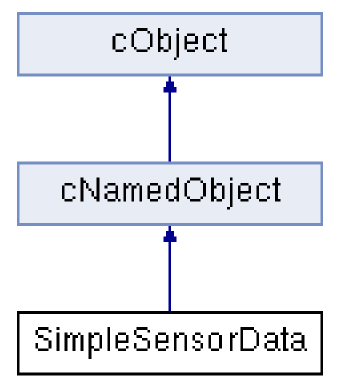
\includegraphics{SimpleClasses}
\end{figure}

\begin{lstlisting}[language=C++, label=lst:SimpleExample]
//im Sender:
cMessage *msg = new cMessage(msgname);
SimpleSensorData *data = new SimpleSensorData("Temperature", temp);
msg->getParList().add(coord);

//
// Nachricht uebertragen    
//  
  
//im Empfaenger:  
SimpleSensorData *data = (SimpleSensorData*) msg->getParList().remove("Temperature");
\end{lstlisting}

\subsubsection{ExtendedMessage}

ExtendedMessage erbt direkt von der Klasse cMessage, der Standard-Nachrichtenklasse in Omnet++. Im Grunde stellt cMessage alle benötigten Funktionen bereit. ExtendedMessage ist nur aus dem Grund vorhanden, um zusätzliche Statistiken über Nachrichten erstellen zu können, zum Beispiel wie oft eine einzelne Nachricht weitergesendet wurde.

\begin{figure}[htbp]
\centering
\caption{ExtendedMessage: Vererbung}
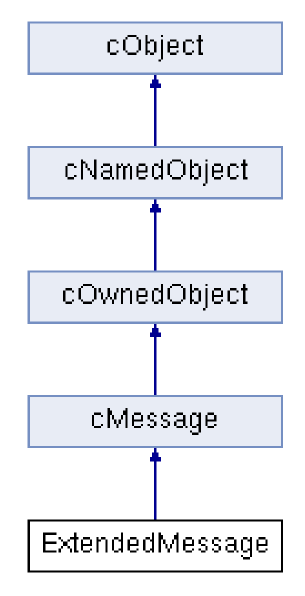
\includegraphics{ExtendedMessage}
\end{figure}

Im Listing \ref{lst:ExtendedMessage} ist zu sehen welche Statistikparameter erhoben werden.

\begin{minipage}{\textwidth}
\begin{lstlisting}[language=NED, label=lst:ExtendedMessage]
message ExtendedMessage extends cMessage
{
	int source;
    int destination;
    int hopCount = 0;    
}
\end{lstlisting}
\end{minipage}

\subsubsection{StatisticsInterface}

Dieses Interface enthält grundlegende Attribute für Statistiken. Klassen die dieses implementieren speichern somit zum Beispiel wie viele Nachrichten sie empfangen oder gesendet haben.


\subsection{Übersicht NED-Module}

Im folgenden Abschnitt werden alle Simulationsobjekte erläutert, also all jene, die durch die Sprache NED beschrieben wurden:

\begin{itemize}{\label{enum:Netzwerk}}
\item Simple Module
\begin{multicols}{2}
\begin{itemize}
\item CustomWorldUtility  
\end{itemize}
\end{multicols}
\item Compound Module
\begin{multicols}{2}
\begin{itemize}
\item bla
\end{itemize}
\end{multicols}
\begin{multicols}{2}
\item Messages
\begin{itemize}
\item ExtendedMessage
\end{itemize}
\end{multicols}
\end{itemize}

\subsubsection{Simple Module}

Simple Module sind Komponenten in einer Omnet++ Simulation, die die größte Auswirkung auf die Wirkungsweise des Netzwerkes haben. Das liegt daran, dass bei ihnen neben einer Beschreibung in NED auch eine Beschreibung in C++ vorliegt. Daher kann das Verhalten jener Module während der Simulation ausführlich definiert werden.

\paragraph{CustomLinearMobility}

Das Modul CustomLinearMobility ist eine Erweiterung der LinearMobility, welche MiXiM bereitstellt. Neben dem Verhalten welches in C++ beschrieben ist, ist das Modul lediglich um den Parameter maxSpeed erweitert, welcher in der omnetpp.ini definiert werden kann.

\paragraph{CustomWorldUtility}

Wie im Codebeispiel (\ref{lst:CustomWorldUtility}) zu sehen ist, ist das Modul CustomWorldUtility eine Erweiterung des Moduls BaseWorldUtility. Zusätzlich zu den darin definierten Eigenschaften hat es einige weitere Parameter. Zunächst eine bool'sche Variable, welche festlegt, ob zu Beginn der Simulation neue Umweltparameter generiert werden sollen. \newline Während numSensorNodes definiert, wieviele Sensorknoten im Netzwerk vorhanden sind und somit wieviele Gates zu Sensorknoten gehen, so definiert numGates die Anzahl der einzelnen Sensoren und somit auch die Anzahl der dahin gehenden notwendigen Gates. Da Sensorknoten auch mit mehr als einem Sensor bestückt sein können, ist der Wert beider Variablen mitunter durchaus verschieden.\newline
Die restlichen Variablen speichern die Umweltparameter in Form einer xml-Datei.

\begin{minipage}{\textwidth}
\begin{lstlisting}[language=ned,caption={CustomWorldUtility},label=lst:CustomWorldUtility]
package mynetwork.WorldModel;
import org.mixim.base.modules.BaseWorldUtility;

simple CustomWorldUtility extends BaseWorldUtility
{
    parameters:
        bool createData;
        int numGates;
        int numSensorNodes;
        xml xmlTemperature = xmldoc("WorldModel/data/temperature.xml");
        xml xmlPressure = xmldoc("WorldModel/data/pressure.xml");
        xml xmlHumidity = xmldoc("WorldModel/data/humidity.xml");
        xml xmlLight = xmldoc("WorldModel/data/light.xml");
        
        @class("CustomWorldUtility");
    gates:
        inout worldDataGate[numGates];
        inout toNode[numSensorNodes];
}
\end{lstlisting}
\end{minipage}

Neben den Parametern besitzt dieses Modul auch noch zusätzlich 2 verschiedene Arten von inout-Gates. Die Menge von worldDataGates verbindet die Welt mit jedem Sensor der auf einem Sensorknoten verbaut ist. Die Menge der toNode-Gates dient für die direkte Verbindung zwischen World und Nodes.

\paragraph{Sensoren}

Es gibt 5 Module welche die Sensoren definieren. Zum einen den allgemeinen Sensor, der das Vatermodul für alle 4 Sensortypen bildet. Er enthält nicht viel, lediglich Gates für Verbindungen zur Welt, um die Umweltparameter abfragen zu können und zum jeweiligen Knoten, für die Kommunikation innerhalb des Bauteils. Weiterhin besitzt er noch einen Parameter, der im Kindmodul den Typ des Sensors beschreibt.

\begin{multicols}{2}
\begin{itemize}
\item HumiditySensor
\item LightSensor
\item PressureSensor
\item TemperatureSensor
\end{itemize}
\end{multicols}

Die 4 Sensortypen, welche vom allgemeinen Sensor erben, definieren jeweils nur den Typ des Sensors. Sie können auf den Knoten als Submodule verwendet werden. Jeder Sensorknoten kann 1 bis 4 Sensoren verschiedener Typen beinhalten und somit ergeben sich 15 verschiedene Arten von Sensorknoten.

\begin{minipage}{\textwidth}
\begin{lstlisting}[language=ned,caption={Sensor},label=lst:Sensor]
package mynetwork.Node.Sensor;

simple Sensor 
{
    parameters:
        //type of the sensor
        string type;
	    @display("i=block/wrx");
	    @class("Sensor");
	gates: 
	    inout toNode;
	    inout worldDataGate;
}
\end{lstlisting}
\end{minipage}

\subsubsection{Compound Module}

Compound Module dienen dazu, andere Module zusammenzufassen, sollen jedoch keine eigene aktive Funktionalität definieren. Ihr Verhalten soll sich allein durch die Submodule ergeben. Es ist daher nicht sinnvoll eine C++-Klasse für diese Module zu definieren.\newline
Alle Sensorknoten, die in dieser Simulation vorkommen sind solche Compound Module.

\paragraph{MyWirelessNode}

Zum einen existiert das Modul MyWirelessNode, welches das Vatermodul für alle Sensorknoten bildet. Es erbt selbst von einem Modul, welches die kabellose Kommunikation unter den Knoten und Batteriestatistiken ermöglicht. Außerdem beinhalten die Knoten auch Funktionen der Mobility, genauer gesagt der CustomLinearMobility, welche auch mobile Knoten ermöglicht. \newline
Es besitzt weiterhin ein inout Gate zur World.

\paragraph{Sensorknoten}

Es gibt insgesamt 15 verschiedene Arten von Sensorknoten, welche am Anfang von Kapitel \ref{enum:Netzwerk} aufgelistet sind. Die Benennung ergibt sich wie folgt (jeweils aus dem Anfangsbuchstaben des englischen Begriffs):
\begin{itemize}
\item T - Temperatur
\item H - Luftfeuchtigkeit
\item L - Licht
\item P - Druck
\end{itemize}
Hierzu ein Codebeispiel des NED-Modules des Knotens, der alle 4 Sensoren enthält: Listing \ref{lst:THLPNode}.

\begin{lstlisting}[language=ned,caption={THLPNode},label=lst:THLPNode]
package mynetwork.Node;
import mynetwork.Node.Sensor.TemperatureSensor;
import mynetwork.Node.Sensor.HumiditySensor;
import mynetwork.Node.Sensor.LightSensor;
import mynetwork.Node.Sensor.PressureSensor;

module THLPNode extends MyWirelessNode
{
    @display("bgb=210,491");
    gates:
        inout toSensor[4];
        inout worldGate[4];

    submodules:
        TemperatureSensor: TemperatureSensor {
            @display("p=140,380");
        }
        HumiditySensor: HumiditySensor {
            @display("p=140,310");
        }
        LightSensor: LightSensor {
            @display("p=140,450");
        }
        PressureSensor: PressureSensor {
            @display("p=70,450");
        }

    connections:
        toSensor[0] <--> { delay = 0ms; } <--> TemperatureSensor.toNode;
        worldGate[0] <--> { delay = measureTime; } <--> TemperatureSensor.worldDataGate;

        toSensor[1] <--> { delay = 0ms; } <--> HumiditySensor.toNode;
        worldGate[1] <--> { delay = measureTime; } <--> HumiditySensor.worldDataGate;
        
        toSensor[2] <--> { delay = 0ms; } <--> LightSensor.toNode;
        worldGate[2] <--> { delay = measureTime; } <--> LightSensor.worldDataGate;
        
        toSensor[3] <--> { delay = 0ms; } <--> PressureSensor.toNode;
        worldGate[3] <--> { delay = measureTime; } <--> PressureSensor.worldDataGate;
}
\end{lstlisting}

Wie man sehen kann erbt der Sensorknoten von MyWirelessNode. Er übernimmt zunächst also alle Eigenschaften des vorher bereits erklärten Modules. Hinzu kommen pro Sensor jeweils 1 Gate zum Sensor und zur world, welches den Sensor mit der Welt verbindet. \newline
Entscheidend für das jeweilige Modul ist jedoch die Definition der Submodule. Im Falle des THLPNode werden genau 4 Submodule definiert:
\begin{itemize}
\item TemperatureSensor
\item HumiditySensor
\item LightSensor
\item PressureSensor
\end{itemize}
Also für jeden Sensor das jeweilige Modul.\newline
Zuletzt werden noch für die Gates die Verbindungen definiert.

\subsubsection{Networks}

Das Netzwerk ist das wichtigste Modul jeder Omnet++-Simulation, denn es fügt alle Elemente zusammen. Ein Netzwerk ist den Compound-Modulen daher nicht unähnlich. 

\paragraph{MyNetwork}

Für das Modul MyNetwork heißt das, dass es eine Instanz des CustomWorldUtility und variabel viele Sensorknoten zusammenfügt, indem es diese als Submodule definiert und deren Gates miteinandern verbindet. Die Definition ist dem MiXiM-Modul BaseNetwork ähnlich, aber hat deutlich mehr zusätzliche Submodule und Parameter. \newline
So sind die Definitionen des Playgrounds, der Mobilität und des ConnectionManager analog, die Submodule der World und des Sensorknoten und die dazu benötigten Parameter, die zum Beispiel die Anzahl der jeweiligen Sensorknoten definieren und die Gateverbindungen jedoch kommen nur hier vor.


Nicht auf den ersten Blick zu erkennen ist die Kommunikation zwischen den Knoten selbst. Die connections sind durch den Term allowunconnected so definiert, dass auch dynamisch Verbindungen aufgebaut werden können, die nicht strikt im Compound Module  definiert sind. Mit Hilfe der sendDirect()-Funktion können so dennoch Nachrichten zwischen Gates versendet werden.

\subsubsection{Messages}

Nachrichten sind das essentielle Werkzeug, um in einem Netzwerk Kommunikation zu ermöglichen. Es gibt ein vordefiniertes Modul cMessage, welches dafür genutzt werden kann. Dieses beinhaltet notwendige Informationen wie zum Beispiel Sendermodul und -gate, Empängermodul und -gate, Sende-, Empfangs- und Erstellzeit und mehr.

\paragraph{ExtendedMessage}

Die ExtendedMessage erweitert diese Funktionalität um einige Informationen für die Statistik.

\begin{lstlisting}[language=ned,caption={ExtendedMessage},label=lst:ExtendedMessage]
message ExtendedMessage extends cMessage
{
    int source;
    int destination;
    int hopCount = 0;    
}
\end{lstlisting}

\subsubsection{omnetpp.ini}

Die omnetpp.ini ist eine Datei, in der Eigenschaften der Simulation geändert werden können, ohne das man den Sourcecode bearbeiten und danach neu kompilieren muss. Es bietet sich daher an, alle Variablen und Konstanten, welche sich öfters ändern hier zu definieren.\newline



Für die relevanten Parameter wurde in der ini-Datei eine spezielle Sektion eingeteilt. Hier können beispielsweise Werte für die playgroundSize vergeben oder festgelegt werden ob Mobilität der Knoten erlaubt sein soll.

\section{Funktionsweise mit Beispielanwendungen}

All die in diesem Kapitel beschriebenen Module wirken für die Simulation zusammen, um ein Netzwerk aus Sensorknoten zu schaffen, in dem die Knoten miteinander und mit ihrer Umgebung gemeinsam agieren können. Dazu werden nach dem Start der Simulation Umweltparameter bereitgestellt und eine festgelegte Anzahl von verschiedenen Sensorknoten erzeugt. Diese können sich anschließend bewegen oder ihr Position beibehalten. Sie können mit ihren Sensoren Werte der Umgebung erfassen und diese über Funk an andere Sensorknoten übertragen, sollte diese in der näheren Umgebung zur Verfügung stehen.
